\documentclass{article}
\usepackage{graphicx} % Required for inserting images

\title{DevOps - LLAMA GEMST}
\author{tbab, harw, gusm, edtr, mihr}
\date{May 2024}

\begin{document}

\maketitle

\section{I'm a section -}
\subsection{I'm a subsection}

\section{Tasks}

\begin{itemize}
  \item Miha, Simon: security analysis
  \item Simon: find \& install template for latex file
  \item Simon: look at Mircea's slides and make us a template for graphs
  \item Tomas: get gh actions to compile latex
  \item Gustave, Eduardo: finish Docker swarm
  \item Eduardo: can you figure out if CodeClimate is installed on repo? if not, install it and give me logins. See session 07 for instructions
\end{itemize}

\section{Introduction}
The following report described the work done during the Spring 2024 DevOps, Software Evolution and Software Maintenance taught at the IT University of Copenhagen. Our report includes the description of the final state of our system, the process we followed to develop and deploy it, lessons we learned, and reflections on technologies used and high and low level decisions we made throughout the semester.

\section{System's Perspective}

A description and illustration of the:

Design and architecture of your ITU-MiniTwit systems
All dependencies of your ITU-MiniTwit systems on all levels of abstraction and development stages. That is, list and briefly describe all technologies and tools you applied and depend on.
Important interactions of subsystems
For example, via an illustrative UML Sequence diagram that shows the flow of information through your system from user request in the browser, over all subsystems, hitting the database, and a response that is returned to the user.
Similarly, another illustrative sequence diagram that shows how requests from the simulator traverse your system.
Describe the current state of your systems, for example using results of static analysis and quality assessments.
MSc should argue for the choice of technologies and decisions for at least all cases for which we asked you to do so in the tasks at the end of each session.

\subsection{How we refactored our app and why we chose GoLang}
\subsection{How a request is processed when it comes from the front-end/simulator}
\subsection{Architecture graphs of the system}
\subsection{List of dependencies (tools and techs) (add some quick description of why we chose a specific dependency if we're not going to write a paragraph about it later in the text)}
\subsection{Db design and cloud db?}
\subsection{Static analysis tool results}

\section{Process' Perspective}

This perspective should clarify how code or other artifacts come from idea into the running system and everything that happens on the way.

In particular, the following descriptions should be included:

A complete description of stages and tools included in the CI/CD chains, including deployment and release of your systems.
How do you monitor your systems and what precisely do you monitor?
What do you log in your systems and how do you aggregate logs?
Brief results of the security assessment and brief description of how did you harden the security of your system based on the analysis
Applied strategy for scaling and upgrades
Also, in case you have used AI-assistants during your project briefly explain which system(s) you used during the project and reflect how it supported/hindered your process.

\subsection{Diagram showing our CI/CD chains, how we release and deploy}
\subsection{How we monitor our systems and what we monitor/how we use this information to improve our system (give the example of indexing the db)}
\subsection{Logging and all that witchcraft crap. What we log and why we used those technologies, how we make sure that we're not logging too little but also not logging too much}
\subsection{Security assessment}
\subsection{Strategy for scaling and upgrading our system (talk about moving to a cloud db, and buying more droplets when moving to swarm}
\subsection{Our use of AI assistants}

\section{Lessons Learned Perspective}

Describe the biggest issues, how you solved them, and which are major lessons learned with regards to: evolution and refactoring operation, and maintenance of your ITU-MiniTwit systems. Link back to respective commit messages, issues, tickets, etc. to illustrate these.

Also reflect and describe what was the "DevOps" style of your work. For example, what did you do differently to previous development projects and how did it work?

\subsection{Issues we ran into:}

\begin{itemize}
  \item Container being killed by the OS on the cloud
  \item Database cleared for some reason every now and then?
  \item Slow db querying
  \item Swarm setup issues
\end{itemize}

\subsection{Maybe talk about how nice it was to have a CD pipeline to work on a project together}

\subsection{What tools we used during the semester, how we divided work, how we shared knowledge?}

\subsection{The three DevOps ways and what we used?}

The Principles of Flow

\begin{itemize}

\item Make Work Visible
  \item Visibility:  In our group we apply the requirement of visibility in our work by defining and sharing our tasks in a common task board in Notion, bellow (by 03-03-2024). This helps us to keep track of the work that needs to be done and be informed what is each team member occupied with.

  \begin{figure}[ht]
    \centering
    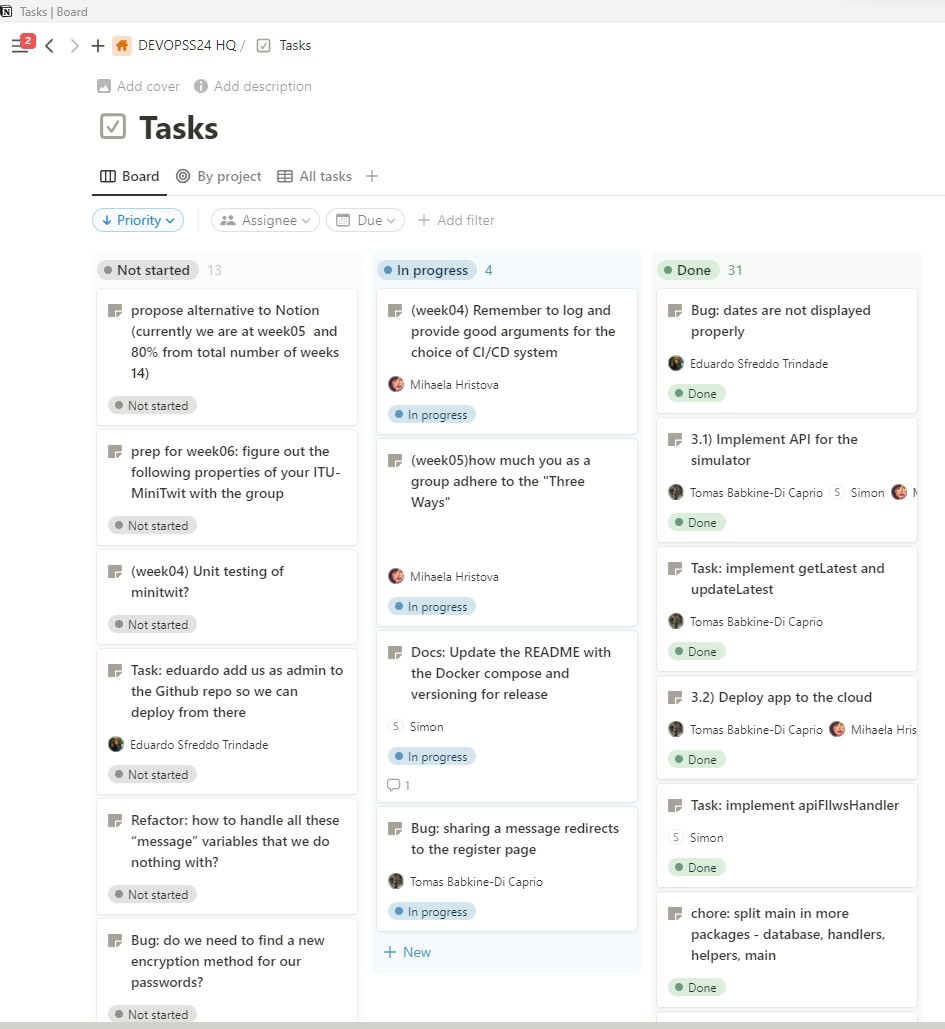
\includegraphics[width=0.8\textwidth]{/home/mihi/DevOps-Adventure/report/report_figures/notion-dashboard-visibility-three-ways.png}
    \caption{Notion dashboard where we keep track of our tasks.}
    \label{fig:notion-dashboard}
    \end{figure}
    
\item Limit Work in Progres
(to be implemented)

We have set a limit of the tasks  that can  be in each column in the Notion board) This means that we can only add a task when one is being finished. In case we are waiting on somebody’s task to be completed and we are free to start new task we will rather see what is causing the delay for our team member to finish his task and help him instead. 

here we could also implement a rule that new week cannot be started without completion of the task for the previous week OR having max three tasks that can be “carried” over.

\item  Reduce batch sizes:

in our case where we develop itu-minitwit application we could look at the different features for example post a message as a single unit operation that is being refactored, tested and deployed with the next *push* to main branch. The idea is instead of  trying to implement all features at once (post messages, follow user, register etc) we develop and test one at a time. This shortens the lead time significantly and most importantly help us to detect and act on bugs much faster.

\item  Reduce the number of hand-offs

Since we are a small organization that consist of 5 members we do not have a risk of wasting time on this principle. However we have implemented CI/CD flow that makes deployment to the cloud automated just with push to main branch. In out deployment process we use configured .yaml file “continuous deployment” that creates VM in Linus server, sets up a docker and tests out application in it (to be implemented), created a docker image of our application that sends to the server provider.

\item Continually Identify and Evaluate Constraints

improve work capacity by following the steps environment creation → code deployment → test setup and run → overly tight architecture

We have detached the dependency from local device by working with VM and Docker where we make sure that all needed requirements to run our application are present. Our deployment process is automated, that is consisted of automated testing of our application on Docker (to be implemented, Postman testing to be mentioned here perhaps? )

We have designed our app architecture with loose couples to achieve independency and safety when implementing changes.

\item Eliminate Hardships and Waste in the Value Stream

/using any material or resource beyond customer requirement is a waste/. Categories of waste: 

-partially done work: all team members are responsible for completion of the task assigned. Even they happen to need help in completion, the initially assigned person has to keep track of the status of the task.

-extra processes: we follow the mandatory assignments that are release each week without trying to develop unrequested features or any other way of deviating of project course work

-extra features: look above

-task switching: we try to keep one person for a task, in case the task is more difficult we might assign more than one person. We do not assign a person to multiple task in case he is unable to complete at least one of them.

-waiting: in case we need to wait for a member to complete his task we always offer help and accelerate the process.

-motion: we meet regularly in person for our lectures and we make sure to have at least one meeting in person per week. When we are not co-located we are distributing our tasks accordingly. Person that is not present gets rather independent task and vise versa. 

-defects: we make sure to be completely informed for a task before we take over.

-nonstandard or manual work: we make sure that nobody is using non-rebuilding servers, test environments and configuration. All our dependencies and operations are aimed to be automatic, self-services and available on demand.

-heroics: unfortunately we cannot ensure that all of our work is happening smoothly and often we depend on each other. This is a common scenario when we have to implement operation or a feature that we are all unexperienced in and we might need another member to give us a green light - for example we have enabled revision/review of the code in our gitHub that requires at least one more member to accept review of the code before we are able to merge. We work on a separate branch each week that is being merged before submission. In case of debug on the main ( for example when implementing CI/CD frow) that required multiple PR and therefore someone else on a stand by to accept the review request (in the middle of the night).

\end{itemize}

\end{document}
